\begin{figure}
  \setlength{\unitlength}{\textwidth}
  \begin{picture}(1,0.5)(0,0.6)
    
    % % %Parkinson Data 
    \put(0.025,0.95){\includegraphics[width=0.5\unitlength]{../FnP/gnuplot/velocity_amp_collapsed_parkinson.eps}}
    \put(0.495,0.95){\includegraphics[width=0.5\unitlength]{../FnP/gnuplot/velocity_amp_collapsed_re165.eps}}
       
    \put(0.025,0.69){\includegraphics[width=0.5\unitlength]{../FnP/gnuplot/mean_power_collapsed_prakinson.eps}}
    \put(0.495,0.69){\includegraphics[width=0.5\unitlength]{../FnP/gnuplot/mean_power_collapsed_re_165.eps}}
       

    \put(0.23,0.67){ $c\rho\mathcal{A}U$}
    \put(0.73,0.67){ $c\rho\mathcal{A}U$}
   	
   	\put(0.01,1.075){$\frac{V}{D}$}

   \put(0,0.8){$\frac{P_{m}}{\rho \mathcal{A}U^3 }$}
    \put(0.08,0.96){(a) }
    \put(0.55,0.96){(b)}
    \put(0.08,0.675){(c)}
    \put(0.55,0.675){(d)}
    
  \end{picture}

  \caption{ Velocity amplitude and mean power  as a function of `$c$' (damping constant). (a) and (c)  are calculated using input $C_y$ data at Re=22300 obtained by \cite{Parkinson1964} and present data at three different damping ratios: $\zeta=0.0125$ (\ding{83}), $\zeta=0.015$ (\ding{116}) and $\zeta=0.0175$ (\ding{108}). (b)and (d)  are at Re=165 are calculated  from the fixed body simulations and present data from three different damping ratios: $\zeta=0.075$ ($\times$), $\zeta=0.1$ (\ding{117}) and $\zeta=0.15$ (+). The collapsed data implies that there is no frequency selection and the tuning parameter of the mechanical side of the system is the damping constant to obtain an optimum power output.}
    \label{fig:collpased_data}
\end{figure}

\ %vspace{10cm}
